
\documentclass[Afour,sageh,times]{sagej}
\usepackage{etoolbox}
\usepackage{mathtools}
\pretolerance=100
\tolerance=200 
\emergencystretch=10pt
\usepackage{graphicx}
\usepackage{nccmath}
\usepackage{pdflscape}
%%%%%%%%%%%%%%%%%%%%%%%%%%%%%%%%%%%%%%%%
\usepackage{txfonts}
%%%%%%%%%%%%%%%%%%%%%%%%%%%%%%%%%%%%%%%%
%\usepackage[options]{hyperref}
% To add links in your PDF file, use the package "hyperref"
% with options according to your LaTeX or PDFLaTeX drivers.
%

\usepackage{fancybox, graphicx}

\usepackage{epstopdf}
\usepackage{hyperref}
\usepackage{xcolor}
\usepackage{rotating}

\usepackage{subcaption}
\captionsetup{compatibility=false}

\hypersetup{
    colorlinks,
    linkcolor={blue!50!black},
    citecolor={blue!50!black},
    urlcolor={blue!80!black}
}
\usepackage{pgfplotstable}
\newcommand{\sbx}[2][c]{%
  \begin{tabular}[#1]{@{}c@{}}#2\end{tabular}}
  
\usepackage{graphicx}
\usepackage{epstopdf}
%% The amssymb package provides various useful mathematical symbols
\usepackage{amssymb}
%% The amsthm package provides extended theorem environments
 \usepackage{amsmath}
 \usepackage{enumitem}


%% make sure you have the nature.cls and naturemag.bst files where
%% LaTeX can find them

%%%% *** Do not adjust lengths that control margins, column widths, etc. ***
\usepackage{amsfonts}
\usepackage[utf8]{inputenc}
\usepackage{url}
\usepackage{array,booktabs}
\newcolumntype{L}{@{}>{\kern\tabcolsep}l<{\kern\tabcolsep}}
\usepackage{colortbl}
\usepackage{xcolor}
\usepackage{graphicx}
\usepackage{caption}
\usepackage{amsmath}
\usepackage{amssymb}
\usepackage{rotating}
\usepackage{multirow}
\usepackage{arydshln}

\setlength{\tabcolsep}{3pt}

 \usepackage{graphicx,rotating,booktabs}
 \usepackage{framed}

\usepackage{lipsum}

\usepackage{multicol}

\setlength{\columnsep}{0.6cm}

\usepackage{listings}

\definecolor{shadecolor}{rgb}{0.9,0.9,0.9}


\definecolor{airforceblue}{rgb}{0.0, 0.53, 0.74}
\definecolor{asparagus}{rgb}{0.31, 0.47, 0.26}

\lstset{ 
  language=R,                     % the language of the code
  basicstyle=\ttfamily, 
  backgroundcolor=\color{shadecolor},  % choose the background color. You must add \usepackage{color}
  showspaces=false,               % show spaces adding particular underscores
  showstringspaces=false,         % underline spaces within strings
  showtabs=false,                 % show tabs within strings adding particular underscores
  frame=single,                   % adds a frame around the code
  rulecolor=\color{black},        % if not set, the frame-color may be changed on line-breaks within not-black text (e.g. commens (green here))
  tabsize=2,                      % sets default tabsize to 2 spaces
  captionpos=b,                   % sets the caption-position to bottom
  breaklines=true,                % sets automatic line breaking
  breakatwhitespace=false,        % sets if automatic breaks should only happen at whitespace
  keywordstyle=\color{airforceblue},      % keyword style
  commentstyle=\color{gray},   % comment style
  stringstyle=\color{asparagus},      % string literal style
  otherkeywords = {install_github, setup_folders, standardize_photos, build_survey, enter_data, compile_data, calculate_payouts, check_classification, downsize, pre_process, auto_enter_all, annotate_data, simulate_selfreport_network, make_strand_data, fit_latent_network_model, summarize_strand_results, data.frame, center, fit_block_plus_social_relations_model, fit_social_relations_model, strand_caterpillar_plot},
  alsoletter ={_},
  deletekeywords={path, start, stop, ordered, case, colors, order, add, data, mode, distance}
} 

\lstdefinestyle{defFile}
{
            keywordstyle = [2]{\color{green}}
}


\newcounter{framecnt}
\newenvironment{frameenv}[1]
    {\begin{figure}[tb]
    \refstepcounter{framecnt}
    \begin{shaded}
    \renewcommand{\theHfigure}{cont.\arabic{framecnt}}
  
    \textbf{\centerline{Box \arabic{framecnt} --- #1}}
         }
    {\end{shaded}\end{figure}
    }



 \usepackage[switch, modulo]{lineno}
\usepackage{arydshln}
\begin{document}

\runninghead{Sosa, Brook, Pery, Redhead, Ross}

\title{Robust Bayesian modeling of animal networks subject to censoring and sampling biases }

\author{Sebastian Sosa\affilnum{1} ... }

\affiliation{\color{black}\affilnum{1}Department of Human Behavior, Ecology, and Culture, Max Planck Institute for Evolutionary Anthropology. Leipzig, Germany}


\corrauth{Sebastian Sosa}

\email{s.sosa@live.fr}

\begin{abstract}
Animal Social Network Analysis (ASNA) has emerged as a crucial approach, leading to significant progress in theoretical and empirical studies of animal social behavior, social development, genetic factors, fitness impact, epidemiology, animal culture, and social structures. This progress owes much to the development of cutting-edge analytical techniques.
\end{abstract}

\keywords{social networks, animal networks, social interactions, generative models }

\maketitle
\section{Introduction}
\linenumbers

Over the past 50 years, graph theory has become a vital tool in studying natural and artificial systems in various fields like anthropology \citep{apicella2012social}, sociology \citep{Milgram1967}, economics \citep{ter2009applying}, ecology \citep{sosa2021animal}. It applies to both small-scale (e.g., proteomics \citep{ravasz2002hierarchical}) and large-scale (e.g., ecosystems \citep{ulanowicz2014limits}) systems. In the realm of animal sociality research, innovative techniques, such as association indices and pre-network permutations\citep{Whitehead1999, Farine2013, Farine2015a}, have expanded upon traditional graph theory. These methods help address specific challenges in this field, like variations in sampling efforts. However, recent studies have highlighted significant reliability concerns associated with hypothesis testing protocols developped in Animal Social Network Analysis (ASNA)\citep{weiss2021common, Puga2021, Hart2022, Farine2022}. 

These issues involve elevated rates of false negatives (meaning failing to reject a false null hypothesis) and false positives (accepting a false null hypothesis). For instance, in a simulation study by \citet{Puga2021}, they considered a scenario with data biases stemming from the data collection process (like oversampling certain individual categories). They identified false positive rates as high as 60.8\% and false negatives rates ranging up to 36.6\%. Since very few biological data collected in natural settings are entirely free from biases related to the studied system or limitations in sampling, these findings emphasize a common challenge that urgently needs addressing to ensure the reliability of hypothesis testing in ASNA. Several approaches have been proposed since the issues with rates of false positives and negatives were raised. These new methods can be categorized into two types based on were they control for bias within the steps of the ASNA hypothesis testing protocol. In ASNA, there are typically two hypothesis testing protocol steps: 1) Estimating social interaction patterns among individuals, which are quantified within a social network and 2) Testing statistical hypotheses about these patterns.

To achieve the first step, researchers calculate a measure of the tendency for individuals to associate (in undirected behavior) or interact (in directed behavior). This measure is referred to as a social index and is computed for each pair of individuals (dyad). These values are used to create a social network, where each individual is a node, and the social index values represent the strength of the connection (edge weight) between dyad members. In addition, social indices have also the goal to control for sampling effort (i.e. heterogeneity in sampling between individuals). Currently two main types of social index are used: association indices \citep{hubalek1982coefficients, sailer1984proximity} and interaction index. Association indices have been used by behavioral ecologist to estimate the proportion of time that a pair of individuals spends together \citep{whitehead2008analyzing}. The higher the index value, the stronger the association within the dyad. The most used association index so far is the simple ratio index (SRI; Eq. \ref{SRI}), designed for data collected in discrete sampling periods (e.g. gambit of the group, scan sampling). The Interaction Index (Eq. \ref{II}) is primarily utilized by primatologists for data collected during continuous sampling periods, such as focal sampling. This index estimates the rate of social interactions per unit of time (e.g. the total time of focus), as opposed to association indices that are proportion-based. A higher index value indicates a stronger rate of interaction within the dyad. Finally, new approaches based on the Bayesian generative network have recently been proposed to estimate interaction patterns among individuals \citep{hart2023bison, Ross2023JAE}. Also, there hasn't been any testing conducted to assess the reliability of results based on biased data. The lingering question is then whether Bayesian generative networks can outperform sociality indices or not.

\begin{ceqn}
\begin{align}\label{SRI}
	SRI_{ij} = {x_{ij}\over y_{i}+ y_{j}+ y_{ij}+ x_{ij}}
\end{align}
\end{ceqn}
Where $x_ij$ is the number of sampling periods with $i$ and $j$ observed associated, $y_i$ is the number of sampling periods with only $i$ identified, $y_j$ is the number of sampling periods with only $j$ identified and $y_ij$ is the number of sampling periods with $i$ and $j$ identified but not associated.

\begin{ceqn}
\begin{align}\label{II}
	II_{ij} = {x_{ij} \over y_{i}+ y_{j}}
\end{align}
\end{ceqn}
Where $x_{ij}$ represents the overall frequencies or total interaction time, $y_i$ and $y_j$ denote the number of observations or the total observation time for individuals $i$ and $j$, respectively.\\

To achieve the second step, which involves testing statistical hypotheses about social interaction patterns among individuals, researchers often use node-based measures computed on the network of association. These measures are derived from the network and help assess various aspects of an individual's position within the network. However, using node-based measures straightforwardly to test hypotheses about individual associations isn't ideal because each association/interaction is counted twice, once for each individual in the dyad, which violates the assumptions of parametric tests. Therefore, much of the methodological work in ASNA has focused on developing techniques to enable valid hypothesis testing. Since 2000, in ASNA permutations have been the main standard coming in two forms: network permutations, pre-network permutations \citep{Farine2013}. For more detailed information on the principles of permutation approaches, readers can refer to \citep{Farine2013, sosa2021reliable}. Issues related to false positive and negative rates were originally demonstrated in network permutations and pre-network permutations. To address these issues, double permutations, which combine both, have been developed and tested on biased data to estimate rates of false positives and false negatives. Double permutations have shown substantial improvement in false positives and false negatives rates compared to other permutation approaches. However, permutations have recently faced criticism for assuming exchangeability of residuals \citep{Hart2022}. Moreover, studies that highlighted problems with permutation approaches or propose new methods have been employing the same simulation protocol and as demonstrated in Appendix 1, this simulation has some issues. Firstly, these simulations were designed to generate "bias of interaction". This bias pertains to missing associations or interactions while observing individuals. It differs from observation bias, as the heterogeneity of observation among individuals is known by the observer(s) and is used by indices of sociality to control for it. In contrast, bias of interaction is unknown to the observer. However, during simulation, generating bias of interaction inadvertently leads to observation bias. This complicates the separation of the effects of both biases and the estimation of which aspects are controlled by indices and/or permutation approaches. 

To tackle these concerns, we developed a new simulation that allows to independently specify sampling bias and interaction bias. Using this simulation, we created various scenarios to assess the reliability of results obtained through different methods: association index, interaction index, Bayesian generative network, network permutation, double permutation and two new methods that will be discussed in the methodology section. Through this research, we have multiple goals. Firstly, we aim to assess whether issues related to false positives and false negatives in ASNA methods are associated with observation or interaction biases. We are expecting to observe accurate results for all approches regarding bias of observation but we are also expecting that once interaction bias will be introduce in the simulation all methods will be inacurate as none of them are accounting for such bias type. Our secondary objective is to determine if Bayesian generative networks reliability in terms of providing accurate estimates and/or differences in hypothesis testing. This is particularly important because the reliability of Bayesian generative networks hasn't been addressed yet. Additionally, having good reliability tests for them could enable us to account for interaction bias as they enable consideration of various types of confounding factors, as we will demonstrate through the presentation of one of your approaches. Our final aim is to identify analytical protocols that can yield more reliable results for hypothesis testing in ASNA. Over the years, multiple approaches have been proposed and faced with such a plethora of methods, researchers may encounter difficulties in assessing the strengths and weaknesses of each.

\section{Methods}

\subsection{Modeling animal networks}
In the vast majority of cases, researchers in animal behavior  collect network data in the form of numerical outcomes---i.e., the number of times that ties \emph{were observed}, conditional on the number of times that ties \emph{could have been observed}. For example, researchers may conduct a specific number of observations (scans or focals), and the outcome data $Y_{[i,j]}$ might reflect the number of observations in which directed (e.g., grooming or aggression events) or undirected (e.g., spatial associations) ties from individual $i$ to individual $j$ were observed. In this case, the number of observations is the sampling effort,  an \emph{exposure} variable which strongly---indeed, \emph{proportionally}---influences the outcome variable. Thus, we let the variable $E_{[i,j]}$ be the number of observations in which individuals $i$ and $j$ could have observed engaging in the dyadic behavior of interest. As such, a Bayesian model of the network data will generally take the form:  

\begin{ceqn}
\begin{align}\label{maineq}
	Y_{[i,j]} &\sim \mathrm{Binomial}\Big(E_{[i,j]}, \phi_{[i,j]} \Big)
\end{align}
\end{ceqn}

where $\phi_{[i,j]}$ is the \emph{true} latent directed connection strength between $i$ and $j$, represented as the probability that a directed tie from $i$ to $j$ occurs in a given observation. 
$Y_{[i,j]}$ is typically a count of events or duration summed over all scans in the study. 
$E_{[i,j]}$ is the number of observations in which ties between $i$ and $j$ could have been detected \citep[e.g., the total number of scans or the sum of focals for individuals $i$ and $j$.][]{Farine2015a}. Note that in the generative context, $\phi$ represents a true \emph{biological} phenomenon, whereas the outcome variable, $Y$, and the exposure variable, $E$, may be strongly affected by the sampling protocol, researcher behavior, and features of animals $i$ and $j$ other than sociality (e.g., cryptic coloration might cause the researcher to fail to observe true ties). 

The goal of modeling, is to measure $Y$ and $E$, and then recover $\phi$. This can be complicated, however, if there are structural biases in $Y$ and/or $E$. Here, we will consider two potential causes of bias: (1) sampling bias, where features of $i$ and $j$ influence $E_{[i,j]}$, and (2) detection bias, where features of $i$ and $j$ influence measurement of $Y_{[i,j]}$ given $E_{[i,j]}$ independent of $\phi_{[i,j]}$. 

We will now build up a Bayesian model of the data generating process. We will start by describing the sub-model underlying the true weighted network of ties, and then integrate the sub-models underlying the measurement process.

\subsection{Social relations}
\subsubsection{Model definition}

We begin the process of building up the model described in Eq. \ref{maineq} by providing a generative model for the \emph{true} latent directed connection strength between individuals $i$ and $j$, $\phi_{[i,j]}$. In order to generate  networks with empirically plausible typologies, it is generally necessary to define a model for $\phi_{[i,j]}$ that includes correlated random effects for the propensity to send and receive ties (nodal random effects), and correlated dyad-level random effects for the propensity of $i$ to send to $j$ and $j$ to send to $i$. Additionally, such models should permit inclusion of covariate effects that influence block/group structure, node-level tie propensity, and dyad-level tie propensity. See Fig. \ref{examplenet} for an example network generated under such a model.

Following prior work of \citet{redhead2021reliable, ross2022modelling}, we recommend the use of the social relations model \citep{kenny1984social, snijders1999social, back2010social} with an additional set of stochastic blockmodel parameters \citep{holland1983stochastic, karrer2011stochastic, peixoto2019bayesian} to account for group structure when necessary. As such, $\phi_{[i,j]}$ can be modeled as:
\begin{ceqn}
\begin{equation}\label{link}
\text{logit}(\phi_{[i,j]}) = \alpha + \lambda_{[i]} + \pi_{[j]} + \delta_{[i,j]} + \Gamma(i,j,V) + \ldots 
\end{equation}
\end{ceqn}
where $\alpha$ is an intercept term, $\lambda$ is a vector of individual-specific focal/sender/nominator effects, $\pi$ is a vector of individual-specific target/receiver/nominee effects, $\delta$ is a matrix of dyadic effects, $\Gamma(i,j,V)$ is a function giving an intercept offset as a function of group/bock structuring variables, and the ellipsis signifies any linear model of coefficients and focal, recipient, or dyadic covariates. 

For example, if $S$ is an animal-specific measure, like body size, and $Q$ is a dyad-specific measure, like a matrix of relatedness ties, then the ellipsis  may be replaced with:  $\kappa_{[1]}S_{[i]} + \kappa_{[2]}S_{[j]} + \kappa_{[3]}Q_{[i,j]}$, to give the effects of body size on the probability of sending ties to any target and receiving ties from any target, and the effects of kinship on the probability of dyadic ties.

%To model block structure, we can consider a list of $V$ categorical variables describing individuals $i$ and $j$. Let $B_{[v,b_1,b_2]}$ be a three-dimensional parameter array, %where $v$ run over variables, and $b_1$ and $b_2$ run over the category levels within variables. Finally, let the function  $b(i,v)$ return the block of individual $i$ for variable %$v$. Then, we can define $\Gamma(i,j,V)$, such that: 
%\begin{ceqn}
%\begin{equation}\label{link}
%\Gamma(i,j,V) = \left(\sum_{v=1}^{V} B_{[v,b(i,v),b(j,v)]} \right)
%\end{equation}
%\end{ceqn}
%where the probability of a tie from individual $i$ in block $b(i,v)$ to individual $j$ in block $b(j,v)$ for variable $v$ is controlled by the corresponding entry in the array of %block parameters, $B_{[v,b(i,v),b(j,v)]}$.\\
% For discrete block modeling, we can utilize the assortativity coefficient: https://arxiv.org/pdf/cond-mat/0209450.pdf

\subsubsection{Priors}
To complete the model definition, we define vague priors. We model the sender and receiver effects jointly using a multivariate normal distribution. This allows for generalized correlations at the individual level to be detected---i.e., we can detect if individuals who groom others are also more likely to be groomed by others. For computational efficiency \citep{stan2021, lewandowski2009generating}, it is best to write the multivariate normal as:
\begin{ceqn}
\begin{equation}
 \begin{psmallmatrix}
\lambda_{[i]} \\
\pi_{[i]}
\end{psmallmatrix}
 =  \begin{psmallmatrix}
\sigma_\lambda\\
\sigma_\pi
\end{psmallmatrix} \circ \left(L* \begin{psmallmatrix}
\hat\lambda_{[i]} \\
\hat\pi_{[i]}
\end{psmallmatrix}\right)
\end{equation}
\end{ceqn}
where $L$ is a Cholesky factor from the decomposition of the $2 \times 2$ correlation matrix with $\rho$ on the off-diagonal, and $\hat\lambda_{[i]}\sim \text {Normal}(0,1)$ and $\hat\pi_{[i]}\sim \text {Normal}(0,1)$ are unit-normal random effects. 
Weakly informative priors may then be independently specified on the variance and correlation terms \citep{lewandowski2009generating}:

\begin{ceqn}
\begin{align}
\sigma_\lambda &\sim \text {Exponential}(1.0)\label{bob69}\\
\sigma_\pi &\sim \text {Exponential}(1.0)\label{bob420}\\
L &\sim \text {LKJ Cholesky}(2.5)\label{bob420L}
\end{align}
\end{ceqn}

We use the above approach to define the dyad-level random effects as well:

\begin{ceqn}
\begin{equation}
 \begin{psmallmatrix}
\delta_{[i,j]} \\
\delta_{[j,i]}
\end{psmallmatrix}
 =  \begin{psmallmatrix}
\sigma_\delta\\
\sigma_\delta
\end{psmallmatrix} \circ \left(L_\delta*  \begin{psmallmatrix}
\hat\delta_{[i,j]} \\
\hat\delta_{[j,i]}
\end{psmallmatrix}\right)
\end{equation}
\end{ceqn}
where $\hat\delta_{[i,j]}\sim \text {Normal}(0,1)$ have unit-normal priors, and the variance and correlation terms have weakly informative priors:

\begin{ceqn}
\begin{align}
\sigma_\delta &\sim \text {Exponential}(1.0)\label{bob89}\\
L_\delta &\sim \text {LKJ Cholesky}(2.5)\label{bob89L}
\end{align}
\end{ceqn}

Under this model, $\rho_\delta$ provides a measure of dyadic reciprocity---i.e., whether the probability of focal $i$ giving to alter $j$, increases with the probability that focal $j$ gives to alter $i$.

We recommend standardizing predictor variables. We can then use weakly regularizing priors on the $\kappa$ terms:
\begin{ceqn}
\begin{align}\label{booyaaaa}
\kappa_{[p]} \sim \text{Normal}(0, 1)
\end{align}
\end{ceqn}

%Lastly, the diagonal elements of $B_{[v]}$, which control the frequency of ties within blocks, will generally have slightly higher prior weight than the off-diagonal elements, %though other topologies are possible \citep[see][]{batagelj1997notes}. For example, we might write:
%\begin{ceqn}
%\begin{align}
%	\beta_{k \to k} &\sim \mathrm{Normal}\Big( \text{Logit}\Big(\tfrac{0.1}{\sqrt{N_{[k,v]}}}\Big) , 2.5 \Big)\label{eq1zz1} \\
%	\beta_{k \to \tilde k} &\sim \mathrm{Normal}\Big( \text{Logit}\Big(\tfrac{0.01}{0.5\sqrt{\vphantom{N_{\tilde k}}N_{[k,v]}}+0.5\sqrt{\vphantom{N_{\tilde k}}N_{[\tilde k,v]}}}%\Big) , 2.5 \Big)\label{eq1zz2}
%\end{align}
%\end{ceqn}
%
%Here, $k \to k$ indicates a diagonal element and $k \to \tilde k$ indicates an off-diagonal element. 
%The scalar of 0.1 in Eq. \ref{eq1zz1} places higher prior density on the diagonal of $B$ (which controls the probability of within-block ties), than the off-diagonal of $B$ (where %the scalar of 0.01 from Eq. \ref{eq1zz2} generates reduced prior between-block tie probability). 
%The scalars of $\sqrt{N_k}$ ensure that prior tie probability scales with sample size at roughly the same rate that we see in empirical data sets \citep{powerready2021}. 
%The standard deviation of 2.5 in both equations causes the overall prior to be quite weak,  and thus allows the data to dominate the posterior. 
%These priors, and all other default priors discussed below, however, can be modified by the user according to their needs by passing in a labeled list of priors when calling the model function.

\begin{figure*}[t]
\caption{Simulated animal network data under the generative model described in \citet{ross2022modelling}. Nodes are colored by group. The stochastic block model introduces gross substructure, where ties within-groups are more likely than ties between groups. These rates can be varied continuously, producing networks with no group structure on one extreme, to networks fully segmented by group identity on the other. Random effects for sending and receiving ties lead to variable degree. Here, some individuals have small degree and are connected to the network by only a single tie, and others have a high degree and are connected to many other individuals. As with the parameters controlling group structure, the parameters controlling variance (and covariance) in individual-level propensity to send and receive ties can be varied continuously, producing networks with approximately uniform degree on one extreme, to networks with highly unequal degree distributions on the other extreme. Finally, we note that some dyads form reciprocal ties (note the black, bidirectional arrows), while other dyads are linked only by unidirectional ties (note the grey, unidirectional arrows). The parameters controlling variance (and covariance) in dyadic random effects, are continuously variable, and can produce networks with close to no dyadic tie reciprocation on one extreme, and networks with high rates of tie reciprocation on the other.   }\label{examplenet}
\centering
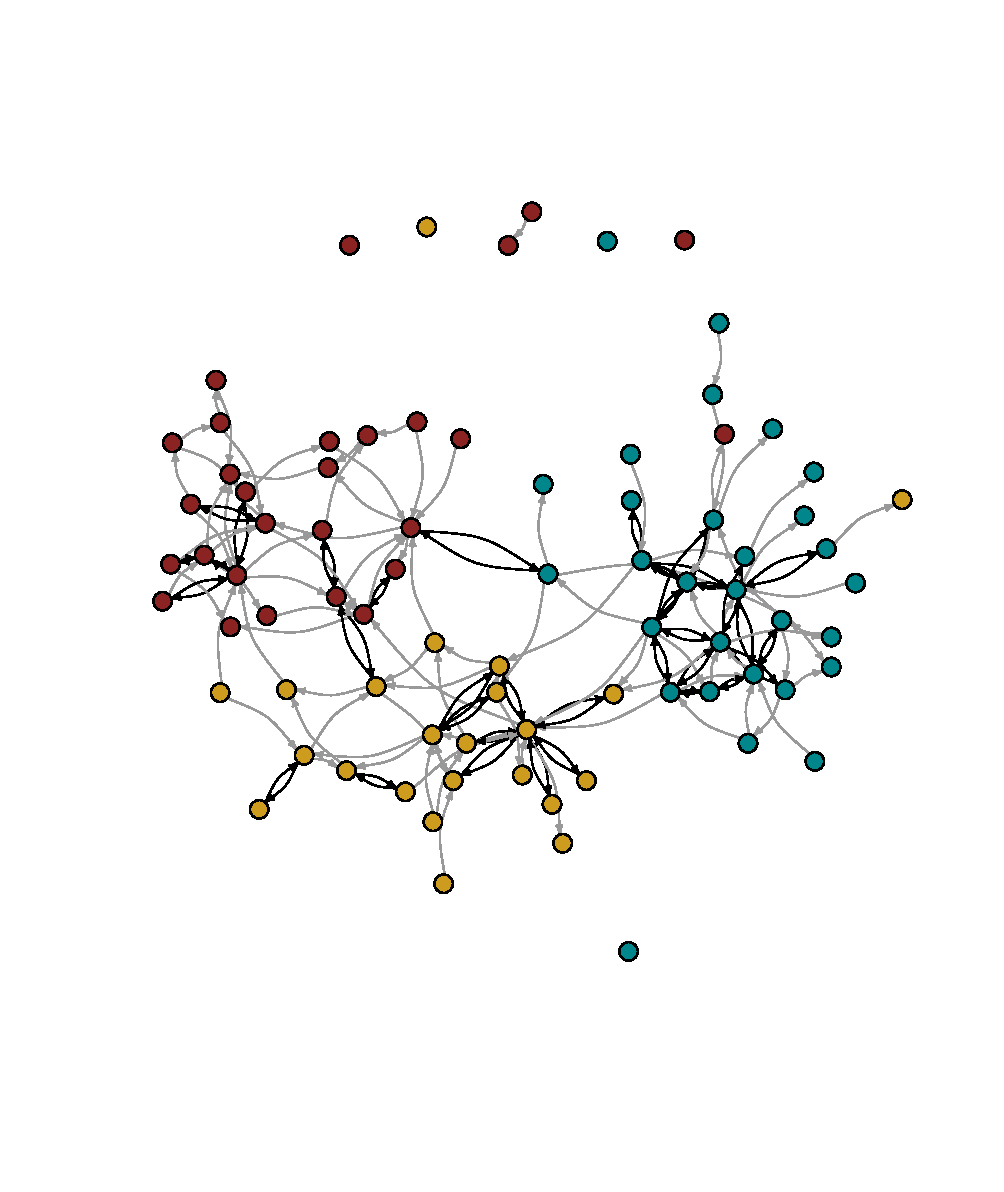
\includegraphics[trim={0 5cm 0 4.4cm},clip,width=0.9\textwidth]{Figures/Example}
\end{figure*}

\subsection{Sampling bias}
The next step in building the model described in Eq. \ref{maineq}, is to provide a generative model for the sampling effort between individuals $i$ and $j$, $E_{[i,j]}$. Most data collection protocol designs can be separated in two categories: discrete time sampling rule and continuous recording sampling rule \citep{bateson2021measuring}. Discrete time sampling rule are instantaneous or one-zero sampling such as "gambit of the group" or "scan" sampling protocol (See \citet{sosa2021reliable} for further details) which involves behavioral events without duration collected through "snapshots". In such data collection protocol, the sampling effort of an individual $i$ would be the count of sampling periods during which it was observed. Continuous recording sampling rule are behavioral state with (e.g., time of grooming) or without (e.g., frequencies of grooming) duration collected with focal sampling protocol.The sampling effort of an individual $i$ would be the time of all focal bouts made on $i$. Wether for discrete or continuous recording sampling a simple model of sampling effort can be written as:

\begin{ceqn}
\begin{align}\label{eq2}
	\hat E_{[i]} &\sim \mathrm{Binomial}\Big(\bar E, \epsilon_{[i]} \Big)
\end{align}
\end{ceqn}

where $\bar E$ is maximum sampling effort (i.e., the count of observations for individual $i$, either as the number of scans or the number of focals), $\hat E_{[i]}$ is the realized number of scans or focals of individual $i$, and $\epsilon_{[i]}$ is the probability that individual $i$ is observed from the researcher. The parameter $\epsilon_{[i]}$ might vary as a function of individual-level characteristics, that also influence network structure. For example, an animal with a cryptic phenotype may be more likely to be unobserved---even as the focal in a focal-follow---if their coloration allows them to escape the attention of the researcher performing the behavioral observation. Similarly, individuals with a cryptic phenotype may be under-sampled, because they are less likely to be found on a given day, and are thus subject to fewer focal follows than desired overall. 

\begin{ceqn}
\begin{align}\label{eq2b}
\text{logit}(\epsilon_{[i]}) = \nu_{[0]} + \ldots 
\end{align}
\end{ceqn}
where $\nu_{[0]}$ is an intercept, and the ellipsis signifies any linear model of coefficients and individual-level covariates. For example, if $S$ is an animal-specific measure, like a binary variable for cryptic coloration, then the ellipsis  may be replaced with:  $\nu_{[1]}S_{[i]}$, to give the effects of coloration on number of scans. 

Then, following standard approaches \citep[e.g.,][]{Farine2015a}, the dyad-level count of scans is given by the formula:
\begin{ceqn}
\begin{align}\label{eq2c}
E_{[i,j]} = \hat E_{[i]} + \hat E_{[j]} 
\end{align}
\end{ceqn}
as ties between $i$ and $j$ can be detected either when $i$ is subject to observation or when $j$ is subject to observation.

From our formalization, it is obvious that variation in sampling effort should have little to no effect on our ability to identify accurate estimates of $\phi_{[i,j]}$ from Eq. \ref{maineq}, as long as we apply statistical methods that propagate uncertainty according to the rules of probability theory. A binomial model of $Y_{[i,j]}$ given $E_{[i,j]}$ provides information about expected value of $\phi_{[i,j]}$ that does not depend on $E_{[i,j]}$; however, the narrowness of the posterior distribution of $\phi_{[i,j]}$ does depend on $E_{[i,j]}$, as we can be more confident in estimates of $\phi_{[i,j]}$ that are based on more observations.

\subsection{Interaction bias, or censoring}
Censoring, or ``interaction bias'' is a more severe problem. In this case, a researcher performed $E_{[i,j]}$ scans and detected $\hat Y_{[i,j]}$ ties. However, if he or she is following animal $i$, and animal $j$ has a cryptic phenotype, then it is possible that ties from $i$ to $j$, or $j$ to $i$,  did occur, but the researcher did not detect them. For a single observation, the indicator of a true tie be $Q_{[i,j]} \in\{0,1\}$, the indicator of a detected tie be $\hat Q_{[i,j]}\in\{0,1\}$, and the indicator for individual $i$ being detectable be $D_{[i]}\in\{0,1\}$. Then, we find that:
  \begin{equation}\label{mixy1}
    Pr[\hat Q_{[i,j]}=0] = Pr[(1-Q_{[i,j]})D_{[i]}D_{[j]}] + Pr[1-D_{[i]}D_{[j]}]
  \end{equation}
  \begin{equation}\label{mixy2}
    Pr[\hat Q_{[i,j]}=1] = Pr[Q_{[i,j]}D_{[i]}D_{[j]}]
  \end{equation}
  where zeros arise as a mixture of two process: (1) a process where both $i$ and $j$ were detectable, but no tie occurred, and (2) a process where either $i$ or $j$ was censored; ones, however, can only occur when both $i$ and $j$ were detectable and a true tie occurred. 
  
Let $\eta_{[i]}=Pr[D_{[i]}=1]$ describe the detectability of individual $i$ and $\phi_{[i,j]}=Pr[(1-Q_{[i,j]})]$. We note that Eqs. \ref{mixy1} and \ref{mixy2} define the probability mass function of a Bernouli random variable, and so we can aggregate over scans, $E_{[i,j]}$, to yield a Binomial model. Thus, we can rewrite Eq. \ref{maineq} as:

\begin{ceqn}
\begin{align}\label{maineq2}
	\hat Y_{[i,j]} &\sim \mathrm{Binomial}\Big(E_{[i,j]}, \phi_{[i,j]}\eta_{[i]}\eta_{[j]} \Big)
\end{align}
\end{ceqn}

We can let $\eta_{[i]}$ depend on individual-specific covariates:
\begin{equation}\label{mixy2}
\text{logit}(\eta_{[i]}) = \psi_{[0]} + \ldots 
\end{equation}

where $\psi_{[0]}$ is an intercept, and the ellipsis signifies any linear model of coefficients and individual-level covariates. For example, if $S$ is an animal-specific measure, like a binary variable for cryptic coloration, then the ellipsis  may be replaced with:  $\psi_{[1]}S_{[i]}$, to give the effects of coloration on detectability.

Here, however, we run up against the limits of inference. Since $\phi_{[i,j]}$ and $\eta_{[i]}$ multiply, the likelihood cannot distinguish between effects, of $S_{[i]}$ for example, that increase the odds of a tie and effects that increase the odds of detectability.

The only way to permit accurate inference, is to use an independent source of data to anchor estimation of $\eta_{[i]}$. If, for example, a researcher conducts $\bar Z_{[i]}$ trials to encounter individual $i$ in a setting where individual $i$ is known to be present, and observes individual $i$ in $Z_{[i]}$ of those trials, this permits inclusion of a model like:
\begin{ceqn}
\begin{align}\label{maineq2}
 Z_{[i]} &\sim \mathrm{Binomial}\Big(\bar Z_{[i]}, \eta_{[i]} \Big)
\end{align}
\end{ceqn}
allowing estimation of social-network parameters that are robust to censoring, or 'interaction bias'.

\subsection{Testing ASNA methods}
\subsubsection{Scenarios:} 
Using the previously explained simulation model, we generated six types of scenarios. Scenario 1, we simulated data where individuals' characteristics have no effect on their social ties and without sampling or censoring biases. This will allow to assess rates of false positives for each approach tested. Scenario 2, we simukated data where individuals' characteristics have an effect on their social ties and without sampling or censoring biases. This will allow to assess rates of false negatives for each approach tested. 
In Scenario 3, we simulated data where individuals' characteristics have no effect on their social ties, introducing sampling bias but without censoring biases. This helps assess rates of false positives for each approach tested in the presence of sampling biases. In Scenario 4, data simulation includes individuals' characteristics affecting social ties with sampling biases and no censoring biases, allowing us to assess rates of false negatives for each approach tested under sampling biases conditions. In scenario 5, we simulated data where individuals' characteristics have no effect on their social ties, introducing censoring biases without sampling biases. This helps assess rates of false positives for each approach tested in the presence of censoring biases. In scenario 6, data simulation includes individuals' characteristics affecting social ties without sampling biases and with censoring biases, allowing us to assess rates of false negatives for each approach tested under censoring biases conditions. 

For each scenario, we generated 100 simulations with random variations in the simulation parameters related to the effect size of individuals' characteristics on social ties, sampling biases, and censoring bias. Details on the range of parameter variations are presented in Table 1.

\subsubsection{Tested approaches:}
For each simulation, we assessed 5 approaches. Initially, we tested the association index without permutations, along with network and double permutations. Next, we examined the interaction index with the same permutation variations. Additionally, Bayesian generative networks modeling interaction observations (e.g., Bison) and link weight probabilities (e.g., STRAND) have been tested. Finally, we introduced a new method using weigthed regression model for association and interaction indices. 
\newline
Indeed, apply association (Eq. \ref{SRI}) or interaction (Eq. \ref{II}) indices to a point-estimates $\dot\phi_{[i,j]}$ models can violate homoscedasticity linear regression assumptions, especially in small samples. This occurs because Eq. \ref{SRI} and Eq. \ref{II} divide out sample size, and provide samples based on sparse evidence disproportionate weight in downstream analysis Fig. \ref{figWhoa}.a. Unlike Bayesian approaches that automatically adjust the influence of each point in proportion to the sample size of observations Fig \ref{figWhoa}.b, regression models assume homoscedasticity. Homoscedasticity implies equal error distribution between data points, leading to similar values in the diagonal covariance matrix  (Eq. \ref{covM1})

\begin{ceqn}
  \begin{align}\label{covM1}
    C = 
    \begin{bmatrix}
      \sigma^2  & 0 & 0 & \cdots & 0  \\
      0 & \sigma^2 & 0 & \cdots & 0\\
      0 & 0 & \sigma^2 & \cdots & 0\\
      \vdots  &  \vdots &  \vdots & \ddots &  \vdots \\
      0 & 0 & 0 & \cdots & \sigma^2 \\
      \end{bmatrix}
  \end{align}
  \end{ceqn}
  Where $C$ is the covariance matrix, Diagonal elements $\sigma^2$ represent the variance of each observation error and they are all the same because errors are identically distributed.

We propose using weighted linear regression that incorporates the sampling effort of each data point into the covariance matrix of errors, providing advantageswhen handling heteroscedastic data  (Eq. \ref{covM2}).

\begin{ceqn}
  \begin{align}\label{covM2}
    C = 
    \begin{bmatrix}
      \sigma_{1}^2  & 0 & 0 & \cdots & 0  \\
      0 & \sigma_{2}^2 & 0 & \cdots & 0\\
      0 & 0 & \sigma_{3}^2 & \cdots & 0\\
      \vdots  &  \vdots &  \vdots & \ddots &  \vdots \\
      0 & 0 & 0 & \cdots & \sigma_{m}^2 \\
      \end{bmatrix}
  \end{align}
  \end{ceqn}
  Where $C$ is the covariance matrix and where diagonal elements $\sigma_{1}^2$ to $\sigma_{m}^2$ are not identical and each observation has its own variance, unlike in Eq.\ref{covM2}.

For each approach in every simulation, we calculated the estimated effect size along with the permuted p-value. This was done to assess the accuracy ofapproach estimations and the correctness of hypothesis testing conclusions, respectively.

\begin{figure}[h]
\caption{Example data on tie strength generated under a model where a covariate $Z$ has a strong positive effect on tie probability, $\phi_{[i,j]}$, but a negative effect on sampling effort, $E_{[i,j]}$. We plot the true dyadic tie strength on the x axis, and the simple ratio index on the y axis.  In frame (a), we see that many points lie along the diagonal (as expected), but there are also strips of points along the horizontal lines at $y=0.0$, $y=0.5$, and $y=1.0$, where the inferred tie strength is not all that reflective of true tie strength. These points correspond to estimates from small samples. Simply plugging in SRI estimates into a downstream regression leads to poor inference, because samples based on few data-points obscure the underlying predictors of tie strength.}\label{figWhoa}\centering

\begin{subfigure}[b]{0.4\textwidth}
         \centering
         \caption{Simple ratio index}
         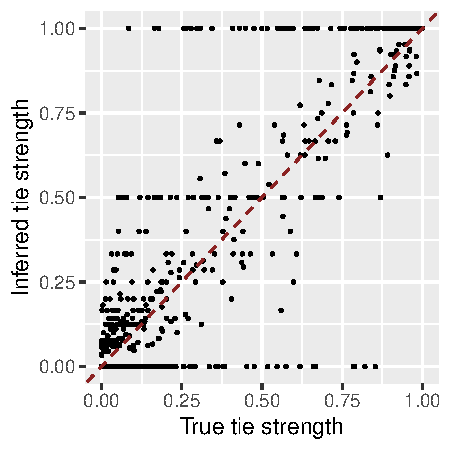
\includegraphics[trim={0 0cm 0 0},clip,width=\textwidth]{Figures/ScatterFrameA.pdf}
         \label{srmx3b_drs}
     \end{subfigure}
     
  \begin{subfigure}[b]{0.4\textwidth}
         \centering
         \caption{A Bayesian model would scale the influence of each point in proportion to the sample size of observations, as we show here by scaling the alpha values of each point by $E_{[i,j]}$. The fact that most of the weight of evidence lies along the diagonal is now much more apparent.}
         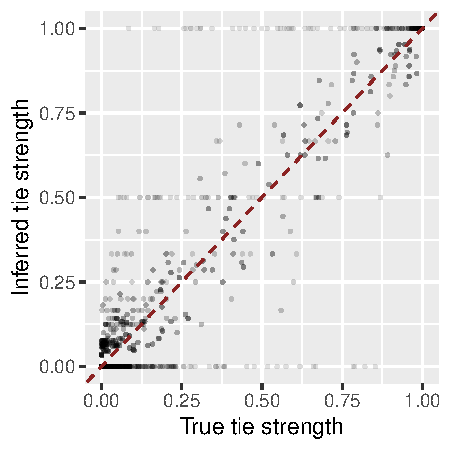
\includegraphics[trim={0 0cm 0 0},clip,width=\textwidth]{Figures/ScatterFrameB.pdf}
         \label{srmx3b_drs}
     \end{subfigure}
\end{figure}

\section{Results}
\subsection{Evaluating the accuracy of the simulation model.}
We assessed the simulation method reliability based on variations in three terms. Initially, we simulated data without any influence of individuals' characteristics on their social interaction patterns, observations, or censoring (Fig. \ref{figSimTest}.A). Next, we simulated data with only an effect of individuals' characteristics on their social interaction patterns (Fig. \ref{figSimTest}.B). Additionally, we conducted a simulation with only an effect of individuals' characteristics on their observations (Fig. \ref{figSimTest}.C). Finally, we performed a simulation with only an effect of individuals' characteristics on their censoring (Fig. \ref{figSimTest}.D). For each simulation type, we used linear regressions to examine the relationship between individuals' characteristics and their social interaction patterns, observations, and censoring, ensuring the reliability of the simulation results. Regression outcomes are summarized in Table 2.

\begin{figure*}[t]
  \caption{XXXX}\label{figSimTest}
  \centering
  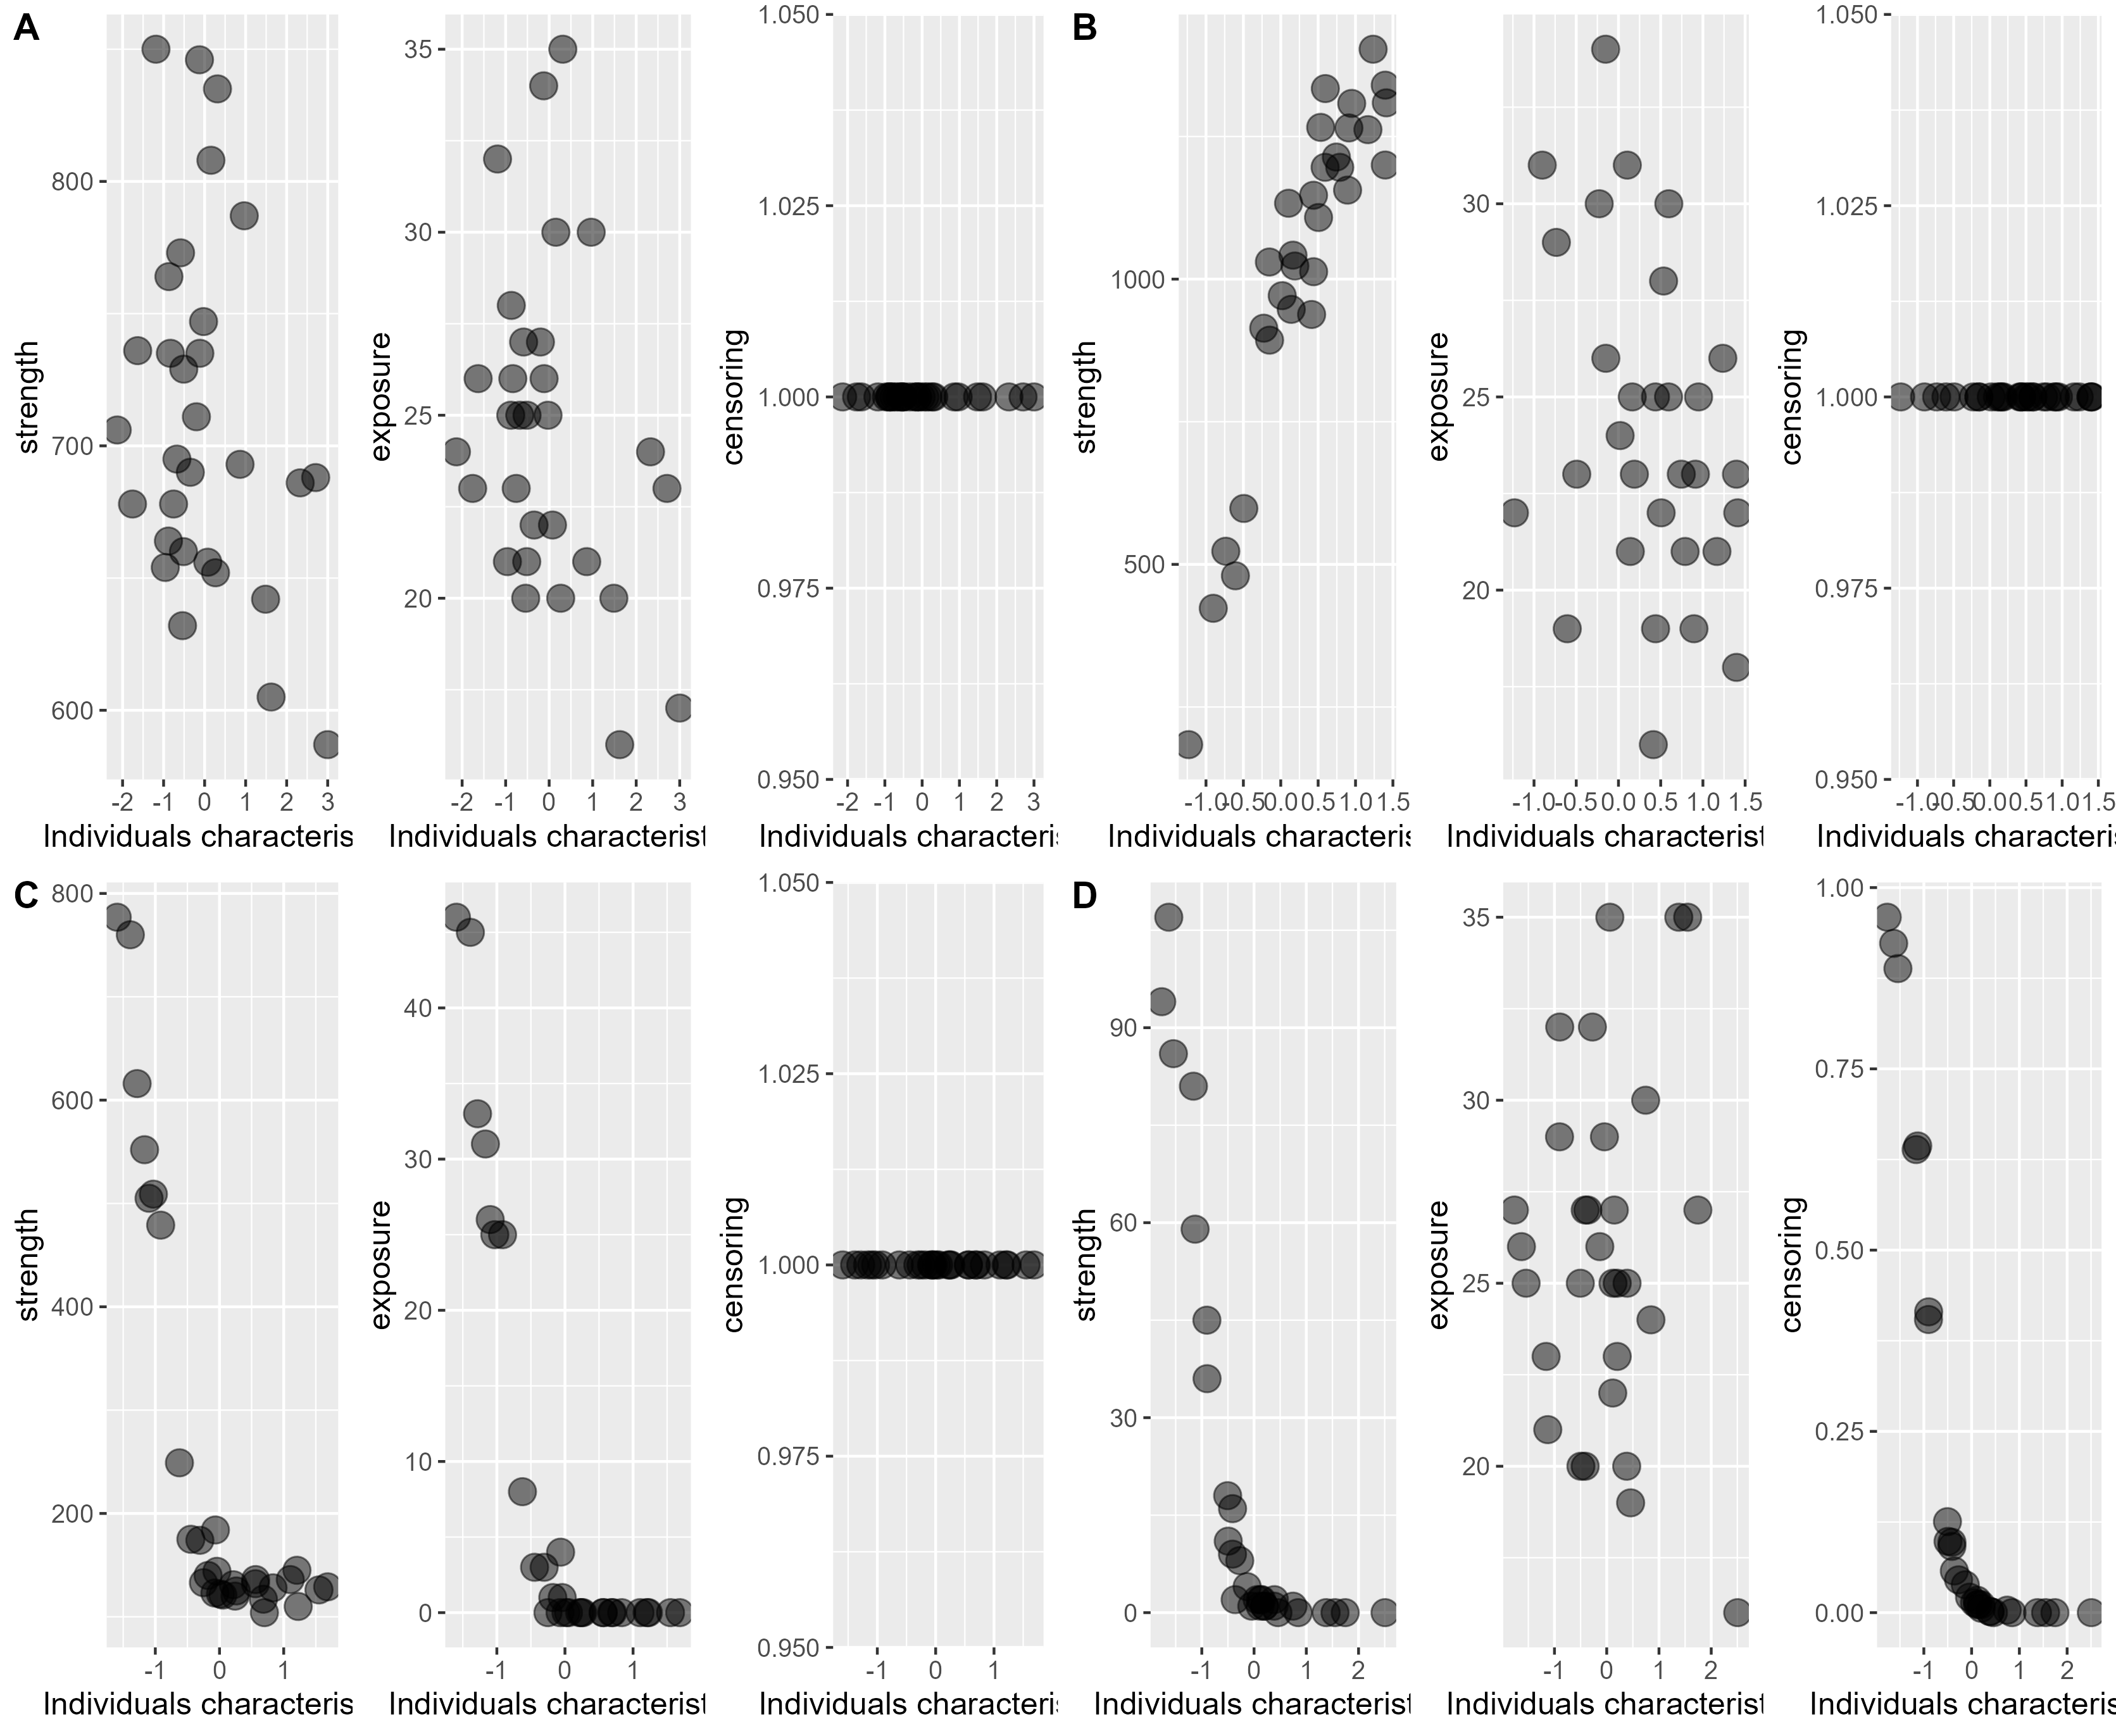
\includegraphics[trim={0 0 0 0cm},clip,width=1\textwidth]{Figures/Appendix2/Figure3.png}
\end{figure*}


\subsection{Scenario 1}

\subsection{Scenario 2}

\subsection{Scenario 3}

\subsection{Scenario 4}

\subsection{Scenario 5}

\subsection{Scenario 6}

\section{Discussion}


\bibliographystyle{SageH}
\bibliography{Final}


\end{document}






Here is a code block:

\begin{minipage}{0.9\linewidth}
\vspace{2mm}
\begin{lstlisting}
# Create the STRAND data object
dat = make_strand_data(
 outcome = outcome,
 block_covariates = block, 
 individual_covariates = indiv, 
 dyadic_covariates = dyad,
 outcome_mode = "binomial",
 exposure = exposure)
\end{lstlisting}
\end{minipage}

At this point, the user must define which outcome model to use. 
The \texttt{STRAND} package supports three outcome modes for each model type: ``binomial'' for proportion data (e.g., if the outcome variable is a matrix containing a count of grooming events between each dyad, and the exposure variable is matrix containing a count of the number of scans in which grooming events between each dyad could have been observed),  ``poisson'' for raw count data (e.g., the number of times constant-time-interval GPS trackers were within 5 meters of each other over a fixed 1-week period),  or finally ``bernoulli'' for binary tie data (e.g., for human self-report/name-generator data, or similar binary tie data from non-human animals).
If the outcome mode is set to ``binomial'', then the \texttt{exposure} variable must be provided. The \texttt{exposure} variable is a labeled list containing a matrix of sample sizes---i.e., counts of the number of times some dyadic tie could have possibly been observed given the sampling protocol.

